\documentclass[tikz,border=2mm]{standalone}
\usepackage{tikz}
\usepackage{pgfplots}
\pgfplotsset{compat=1.18}

\begin{document}
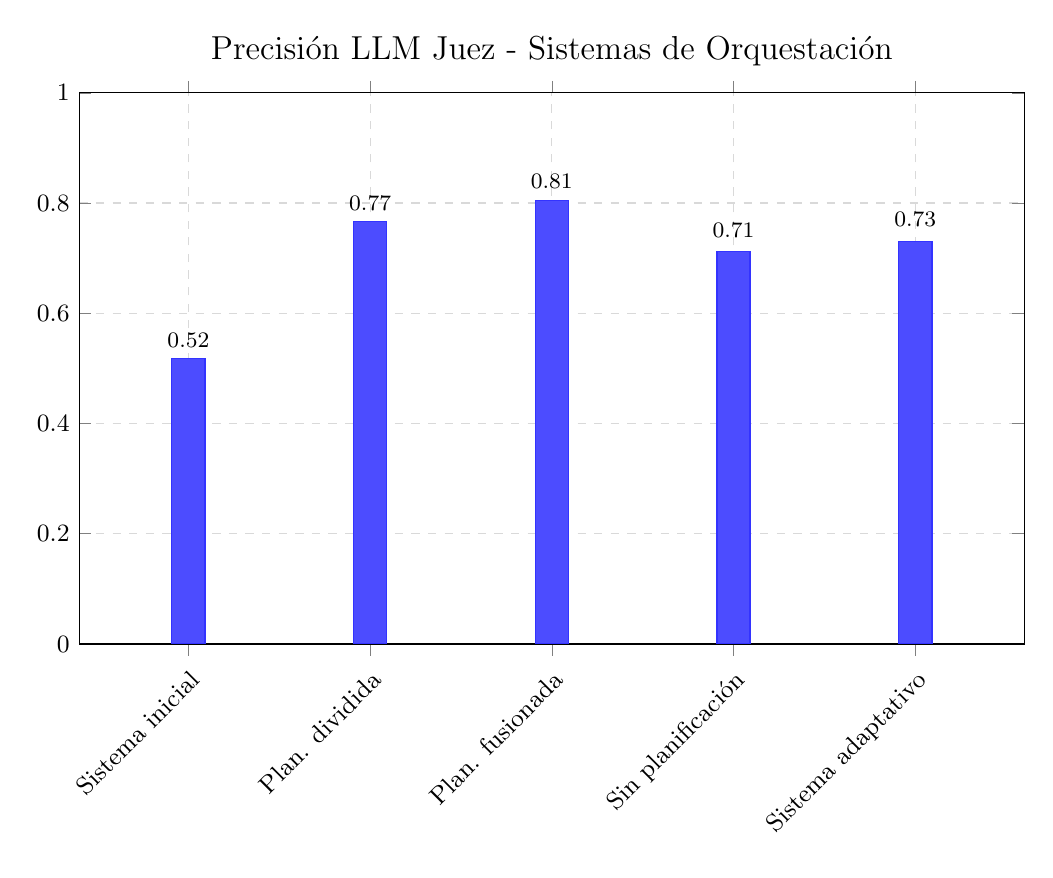
\begin{tikzpicture}
\begin{axis}[
    title={Precisión LLM Juez - Sistemas de Orquestación},
    title style={font=\large},
    ylabel=,  
    xlabel=,
    ymin=0,
    ymax=1.0,
    ytick={0,0.2,0.4,0.6,0.8,1.0},
    enlarge x limits=0.15,
    ybar=4pt,
    bar width=12pt,
    symbolic x coords={Sistema inicial, Plan. dividida, Plan. fusionada, Sin planificación, Sistema adaptativo},
    xtick={Sistema inicial, Plan. dividida, Plan. fusionada, Sin planificación, Sistema adaptativo},
    x tick label style={rotate=45, anchor=north east, font=\small},
    yticklabel style={font=\small},
    width=12cm,
    height=7cm,
    grid=major,
    grid style={dashed, gray!30},
    tick label style={font=\small},
    scale only axis,
]
\addplot[
    fill=blue!70,
    draw=blue!80,
    line width=0.5pt
] coordinates {
    (Sistema inicial, 0.5183)
    (Plan. dividida, 0.7665)
    (Plan. fusionada, 0.805)
    (Sin planificación, 0.7126)
    (Sistema adaptativo, 0.7307)
};

% Añadir valores sobre las barras
\node at (axis cs:Sistema inicial,0.55) {\footnotesize 0.52};
\node at (axis cs:Plan. dividida,0.80) {\footnotesize 0.77};
\node at (axis cs:Plan. fusionada,0.84) {\footnotesize 0.81};
\node at (axis cs:Sin planificación,0.75) {\footnotesize 0.71};
\node at (axis cs:Sistema adaptativo,0.77) {\footnotesize 0.73};

\end{axis}
\end{tikzpicture}
\end{document}
